%\documentclass{article}
%\usepackage[spanish]{babel}
%\usepackage{amssymb, amsmath} %Paquetes matemáticos de la American Mathematical Society
%\usepackage{graphicx}
%\usepackage[%
 %   a4paper,       % Tamaño de papel
%    left=2.5cm,    % Margen izquierdo
%    right=2.5cm,   % Margen derecho
%    top=3cm,       % Margen superior
%    bottom=3cm,    % Margen inferior
%    footskip=1.5cm % Espacio para el pie de página
%]{geometry}
%\usepackage{fancyhdr}
%\pagestyle{fancy}
%\fancyhf{}
%\lhead[\leftmark]{Síntesis de Redes Activas - Laboratorio 1}
%\rfoot[]{\thepage}
%\begin{document}
 \section{Circuito II:  FUENTE DE CORRIENTE CONTROLADA POR TENSIÓN }

\subsection{Esquemático y datos}
Se realiza el análisis teórico del circuito siguiente: 

  \begin{figure}[h!]
     \centering
	 \includegraphics[width=0.4\linewidth]{esquematico2.png}
	 \caption{Esquematico del circuito N° 2}
	 \label{fig:esquematico2}
  \end{figure}
  
  \vspace{1em}
\textbf{Datos:}

\begin{itemize}
  \item Amplificador operacional: LM324
  \item $V_{cc} = 10 \, \text{[V]}$
  \item $V_{ss} = -10 \, \text{[V]}$
  \item $R_1 = 100 \Omega, R_2 = 10k \Omega , R_3 = 1k \Omega , R_4 = 100k \Omega $
\end{itemize}

Este circuito funciona como fuente de corriente, donde independientemente del valor de la carga, la corriente $I_L$ es fija, 
dependiendo solamente del valor de la tensión de entrada aplicada.

\subsection{Análisis teórico}

Considerando que se trata de un amplificador operacional ideal, es decir con $V^+=V^- \quad y \quad A_d = \infty $, y al ser una fuente de corriente controlada
por tensión, los parámetros de interés son $V_{in}, V_o, R_L \quad e \quad I_l$. Luego las corrientes en el nodo de la entrada $V^+$ resultan:

\[ \frac{V_o -V^+}{R_1} + \frac{V_{in}-V^+}{R_3}- \frac{V^+}{R_L}\]

Teniendo
\[ V^+ = V^- = \frac{V_o R_4}{R_4 + R_2}\]

\[V^+ = V^- = \frac{V_o 100k \Omega }{110k \Omega}=0.9 V_o \]

Análisis para $I_{RL}= f( R_L, V_{in}) $ 
 
\[\frac{V_{in}}{R_3} + \frac{V_o}{R_1} = V_0  \frac{R_4}{R_4 + R_2} (\frac{1}{R_L}+\frac{1}{R_1}+\frac{1}{R_3})\]

\[{V_{in}} = V_0  R_3 [ \frac{R_4}{R_4 + R_2} (\frac{1}{R_L}+\frac{1}{R_1}+\frac{1}{R_3}) ] \]

\[{V_{in}} = V_0 [ \frac{1}{R_L}(R_3 \frac{R_4}{R_4 + R_2}) + R_3\frac{R_4}{R_4 + R_2}(\frac{1}{R_1}+\frac{1}{R_3})-\frac{R_3}{R_1} ] \]

Reemplazando con los valores especificados de $ R_1 =100\Omega , R_2=10k\Omega , R_3 = 1k\Omega , y R_4= 100k\Omega$

\[{V_{in}} = V_0 [ \frac{1}{R_L}909,09091] \]


Ahora, sigue la expresión de la corriente que fluye a través de la carga en
función del valor de la carga resistiva y de la tensión de entrada :

\[I_{RL}= \frac{V^+}{R_L}\]
\[I_{RL}= V_o\frac{R_4}{R_4 + R_2} \frac{1}{R_L}\]


\[I_{RL}=\frac{V_{in}}{[\frac{1}{R_L}(R_3{R_4}{R_4 + R_2})]}\frac{R_4}{R_4 + R_2}\frac{1}{R_L}\]

\[I_{RL}= \frac{V_{in}}{R_3}\]

\[I_{RL}= V_{in}.10^{-3}\]

También se puede declarar la amplitud de la tensión de salida en función de la tensión de entrada y de la carga:

\[V_{out} = \frac{V_{in}}{\frac{1}{R_L}909.09091}\]

\[V_{out} = V_{in}R_L.1.1.10^{-3}\]

 \vspace{1em}

Para terminar, se expresará la relación entre el valor máximo de la carga que se puede conectar al circuito y la tensión de entrada. Para determinar la $R_L$ máxima, se debe considerar el caso en el cual Vo sea igual a Vcc (10V):

\[10[V] = V_{in}R_L.1.1.10^{-3}\]
\[R_{L_{max}} = \frac{909.09091}{V_{in}}\]

Calculando los valores de corriente a distintos $R_L \quad y \quad V_{in}$:

\begin{figure}[h!]
     \centering
	 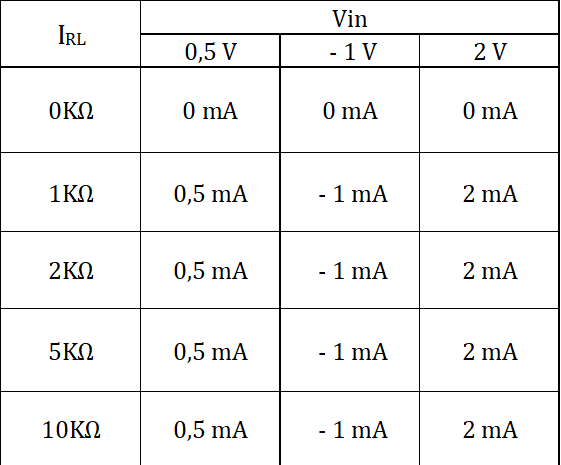
\includegraphics[width=0.45\linewidth]{c2-calculos.png}
	 \label{fig:esquematico2}
  \end{figure}

\subsection{Simulación}

Con la simulación realizada en LTSPice, se completó la tabla con los valores de corrientes según los distintos valores elegidos de la resistencia $R_L$


  \vspace{1em}

\begin{figure}[h!]
 	\centering
 	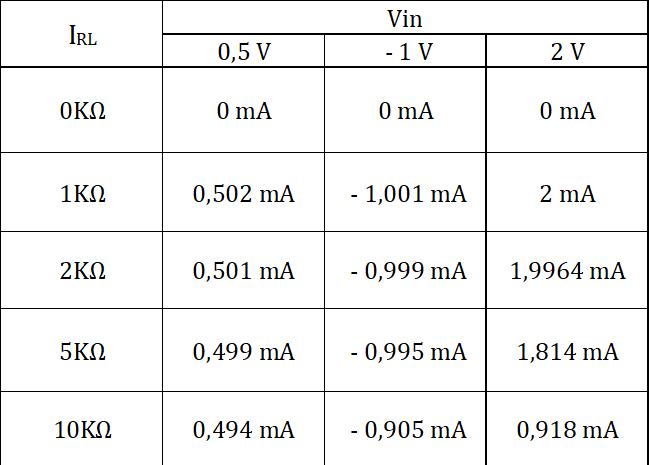
\includegraphics[width=0.5\linewidth]{c2-medicionesS.png}
	 \label{fig:esquematico2}
\end{figure}


%% tensión de entrada?? cuando satura?
Con los datos obtenidos en la tabla anterior se puede notar que son distintos a los calculados teóricamente, ya que al aumentar la resistencia $R_L$, el error de los valores obtenidos aumenta. 
Algo similar sucede cuando se aumenta la tensión de entrada $V_{in}$, el amplificador operacional se satura a 8,49V.

Esto se puede observar en las siguientes gráficas, utilizando distintos valores de tensión de entrada y de resistencia de carga:

  \begin{figure}[h!]
     \centering
	 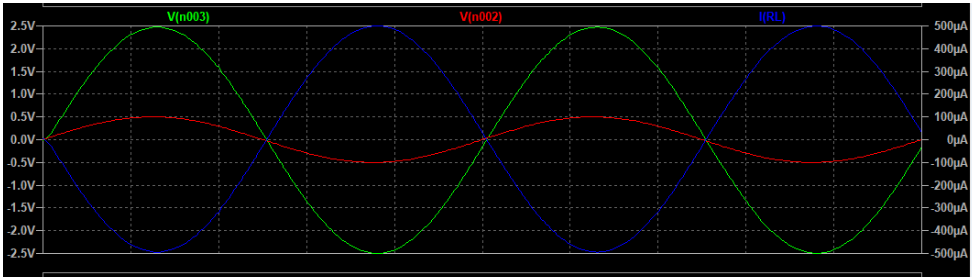
\includegraphics[width=0.7\linewidth]{c2curvasA.png}
	 \caption{$R_L= 5k\Omega, V_{in}= 0.5V, V_o =2.5V $}
	 \label{fig:esquematico2}
  \end{figure}

 \vspace{1em}
 
  \begin{figure}[h!]
     \centering
	 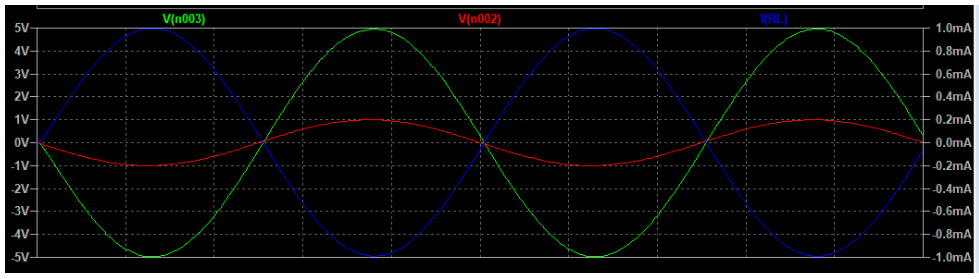
\includegraphics[width=0.7\linewidth]{c2curvasB.png}
	 \caption{$R_L= 5k\Omega, V_{in}= 1V, V_o =5V $}
	 \label{fig:esquematico2}
  \end{figure}
 
  \vspace{1em}
  
 \begin{figure}[h!]
     \centering
	 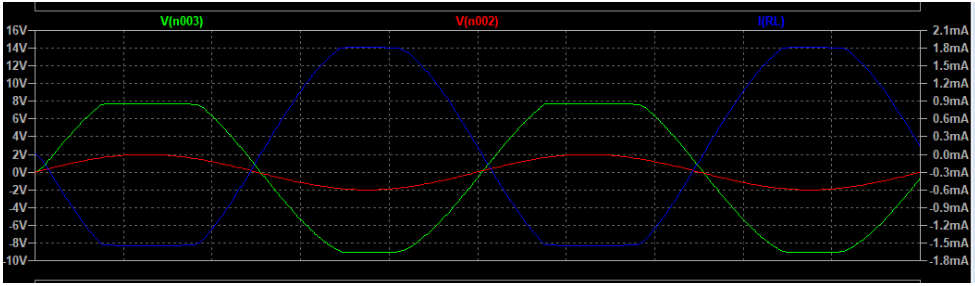
\includegraphics[width=0.7\linewidth]{c2curvasS.png}
	 \caption{$R_L= 5k\Omega, V_{in}= 2V , V_o= 8.4V $}
	 \label{fig:esquematico2}
 \end{figure}
 
 El análisis simulado se aproxima bastante al análisis teórico, siempre y cuando la resistencia de carga no supere en valor a la $R_{Lmax}$ , ya que el AO se saturaría y dismunuiría la corriente de la resistencia de carga.

%\end{document}